\chapter{Conclusion}\label{conclusion}
This work provides important insights into reconfigurable acceleration of transformer neural networks for ultra-low latency applications like high energy physics. The proposed solutions cover the whole development spectrum, from software architecture design, through various optimization techniques, to efficient hardware mapping of the neural network models. In this chapter, the main technical contributions are firstly summarized, followed by a discussion covering the existing limitations discovered during our research. Finally, several possible extensions that could improve upon our work are covered.

\section{Achievements}
This project contributes to the following research areas:

\begin{itemize}
  \item \textbf{Hardware-Aware Neural Network Design}: We explore two neural network architectures, which combine ideas from state-of-the-art solutions and transform them into components that can be efficiently mapped to FPGAs while offering cutting-edge accuracy. The analyzed aspects involve weight and bias fusing for normalization, splitting of fully-connected layers, and preventing numerical instability in softmax activation function. To allow for an easier reasoning about the architectures, analytical models covering latency and DSP slices were developed.

  \item \textbf{Efficient Hardware Mapping}: We propose novel hardware blocks for tensor multiplication using Einstein Notation as well as latency and resource optimized log softmax and SiLU activations. On top of that, we further expand \hlsml library with efficient and customizable self-attention and transformer layers. We also introduce improvements to the fully-connected layer and the unit responsible for storing results of arbitrary precomputed functions. The resulting hardware design achieves nanosecond latency with classification quality comparable to GPU and CPU implementations that are run around thousand times slower.

  \item \textbf{Quantization-Aware Training}: We analyze existing solutions for quantization-aware training and adapt the most suitable framework to transformer neural networks. The conducted experiments highlight the best performing fixed-point representations and highlight potential pitfalls in very complex neural networks.

  \item \textbf{Post-Training Quantization}: We develop a novel algorithm for post-training quantization that can be used with existing models and target any hardware platform. Thanks to its user-defined parameters, the search can be configured to prioritize accuracy over resource utilization or vice-versa. Evaluation on the proposed models results in a nearly \nicefrac{2}{3} reduction of total bit-widths with negligible accuracy decrease.
\end{itemize}

\section{Limitations}
Due to the scope of the project, there was no extensive hyperparameter search involved in any of the neural network architectures. Further tuning might allow for better results, which can have a cascading effect on the rest of this report's analysis because the researched areas are tightly coupled. In other words, more optimized software models lead to better performing hardware implementations, which can be further amplified by carefully quantizing them during or after training. On that topic, the developed post-training quantization algorithm assumes high correlation between subsequent neural network layers. Although this was proven to be the case in our analysis, it might not generalize to every network type.

The more complex of the discussed transformer architectures was not able to be synthesized as a pipelined design using HLS due to the inherent intricacy of generating pipelined models. The serial implementation offers an interesting trade-off of a design that runs slower but requires substantially less resources. However, many real-life applications operate under strict latency constraints, which could not be met due to the existing limitations of the HLS process and the fundamental issue of transformer's complexity.

\section{Future Work}
There are four main areas that our work could be expanded upon, which involve modifying the transformer layer, especially the self-attention mechanism, enhancing the post-training quantization method, adapting existing High-Level Synthesis optimization tools, and experimenting with other datasets.

\subsection{Alternative Transformer Design}
There is an ongoing research into alternative transformer architectures, which improve upon the quadratic complexity of self-attention, that has proven to be the main challenge of accelerating transformers. Some solutions involve low-rank approximations, sparsity, memorization, or various other techniques, summarized in figure \ref{fig:transformer-landscape} \cite{81-tay2020efficient}. To tackle the complexity problem, a recent work also goes as far as exploring completely removing the self-attention layer \cite{82-mikuni2021point}.

\begin{figure}[hpt!]
  \centering
  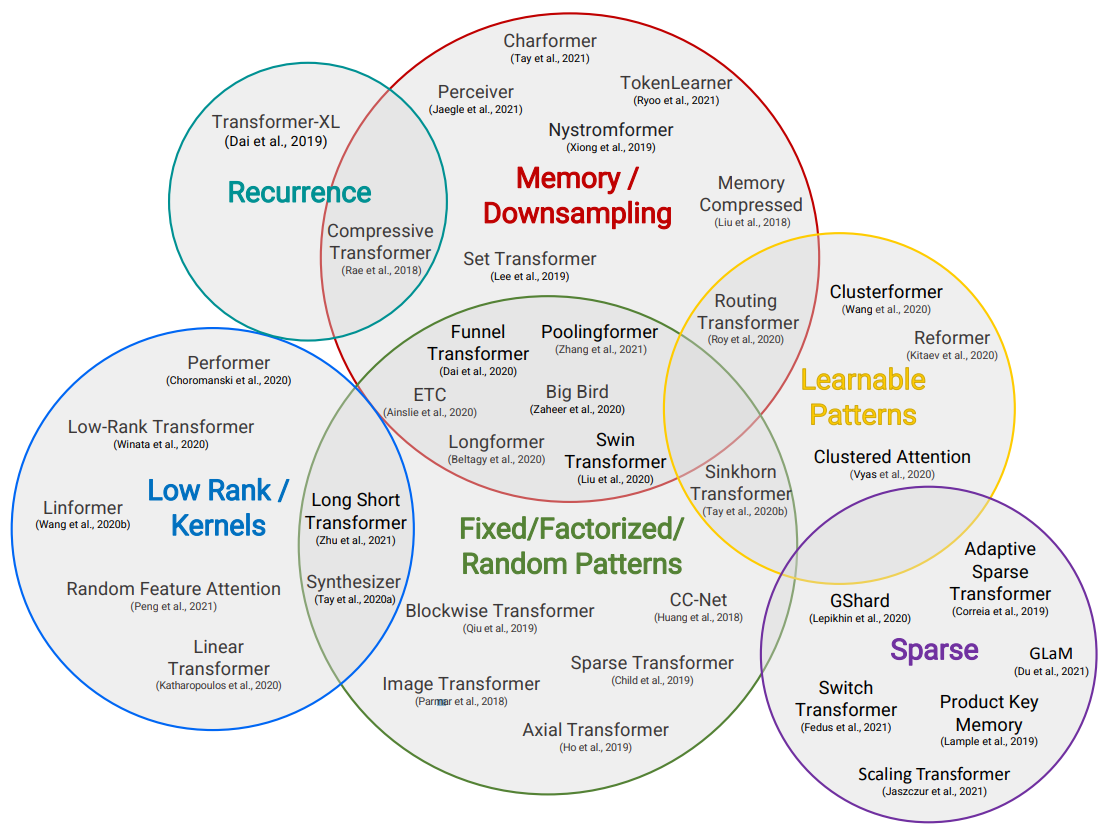
\includegraphics[trim={0cm 0cm 0cm 0cm}, clip, width=0.7\textwidth, center]{conclusion/transformer_landscape.png}
  \caption{Landscape of efficient transformer architectures.}
  \label{fig:transformer-landscape}
\end{figure}

Aside from changes to self-attention, trained transformer models could be compressed using techniques like pruning to decrease the number of stored weights which can improve the inference speed and reduce hardware utilization. Additionally, the already optimized batch normalization layers could be further improved by fusing with linear layers to reduce the overall complexity. Finally, recent automatic methods of finding efficient transformer configurations \cite{83-tsai2020finding,84-su2021vitas:} could help with the hardware-aware architecture search challenge.

\subsection{Post-Training Quantization Advancements}
The proposed post-training quantization algorithm could base its resource estimations on an analytical model to achieve more accurate predictions without compromising the search time. A new metric of energy-consumption could also be taken into consideration to accommodate mobile or embedded platforms' limitations. In order to accelerate the search process while potentially improving its findings, the approach could also benefit from a faster simulation and awareness of tested configurations' positions with regard to the underlying Pareto front or Roofline Model.

\subsection{Automatic High-Level-Synthesis Optimizations}
A recent High-Level Synthesis framework called ScaleHLS \cite{ye2021scalehls} promises to generate efficient RTL designs from HLS C++ or directly from PyTorch thanks to the use of optimizations at different levels of abstraction of the underlying Multi-Level Intermediate Representation (MLIR) \cite{mlir} used for PyTorch \cite{86-llvm2020torch-mlir}. This tool was explored during the project, but similarly to the discussed quantization-aware training methods, it does not support the self-attention layer in case of the direct PyTorch model optimization. As for trying it on the already developed HLS implementation, the size and the deep hierarchy involved in this work exceeds the complexity that ScaleHLS can handle. Nonetheless, further improvements might allow this framework to reduce the development time between designing a transformer architecture using \hlsml and testing its hardware implementation, supporting the objective of this work.

\subsection{Other Datasets}
Both of the datasets used in this project involve classification of five jet categories. However, other examples in the literature often discuss problems with fewer categories, for instance top-tagging, which is an approach to identifying top quarks. Simpler problems are likely to require less complex architectures - an area of the design space that this work proves to be optimal for transformers.

%//////////////////////////////////////////////////////
% at the end, CHECK:
% hyphens,
% 3rd person s in verbs,
% remaining todos,
% ugly page breaks,
% axis and titles in figures,
% correct some references to evaluation to be more specific (find all of them),
% change explanation in (brackets) to footnotes (always?),
% ensure no pre-training quantization but quantization-aware training,
% ensure network names like CNN, TNN are used consistently + no capital letters in convolutional nn, transformer nn,
% check if all hlsml is use with \command
% make all itemize lists use bolded : instead - 